\clearpage
\section[Évaluer SimFeodal]{Évaluer le modèle SimFeodal}

Le modèle SimFeodal présenté dans le chapitre 2 correspond à une \og version 0\fg{} du modèle souhaité, c'est-à-dire qu'il en constitue une première pré-version -- implémentant l'ensemble des mécanismes décidés dans le modèle conceptuel --, qui n'est pas encore stabilisée dans les liens, interactions et valeurs de paramètres de ceux-ci.
Il ne répond donc pas nécessairement aux attentes que l'on peut en avoir.
Si l'on a déjà mentionné des objectifs dans le chapitre précédent (\hl{ref. à ce passage dans, par ex. tableau, dans chap. 2)}, il convient ici de formaliser et d'expliciter le sens de ces attentes.
En effet, celles-si sont hétérogènes, aussi bien dans leur forme que dans l'importance qui leur est accordée, et la description de leurs caractéristiques se révèle importante pour leur mobilisation dans le cadre du paramétrage -- et de l'ensemble des étapes de la vie d'un modèle -- de SimFeodal.
Dans cette partie, on explicitera donc d'abord le sens que l'on prête à ces attentes --indices et indicateurs --, avant de les organiser et de les décrire afin de qualifier le comportement du modèle SimFeodal tel qu'il a été décrit dans le \hl{chapitre 2}.

\subsection{Indices et indicateurs}

On peut caractériser ces dernières, de manière très générale, comme permettant de reproduire les grands traits de cette transition.
La reproduction d'un fait stylisé peut s'entendre de multiples manières, tout au long du gradient qualitatif-quantitatif.
Dans notre cas, en l'absence d'une connaissance quantitative totale des phénomènes mobilisés et observés, on peut s'appuyer sur deux grands ensembles d'\og indices\fg{}.

\subsubsection{Les indices empiriques}

\begin{figure}[H]
	\captionsetup{width=\linewidth}
	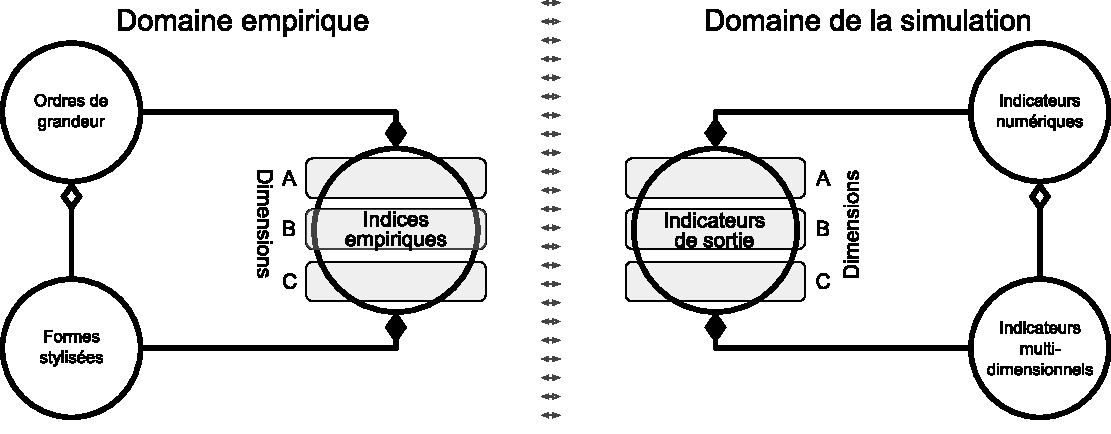
\includegraphics[width=\linewidth]{img/schema_indice_indicateur.pdf}
	\caption{Schéma de synthèse des correspondances entre empirie et simulation pour l'évaluation du modèle SimFeodal.\\ Les losanges pleins désignent une relation de composition : un indice est soit un ordre de grandeur, soit une forme stylisée. Les losanges vides indiquent une relation d'agrégation : une forme stylisée est une agrégation d'ordres de grandeurs.
		\textbf{N.B.} Les termes utilisés ici sont souvent employés pour désigner différents éléments dans la littérature. L'organisation lexicale définie dans ce schéma n'a pour but que d'être explicite quant au sens et à la place donnée à chacun de ces termes dans le présent ouvrage. } 
	\label{fig:schema_indices} 
\end{figure}


\paragraph{Ordres de grandeur}
Le premier est constitué d'\textbf{ordres de grandeurs} empiriques estimés -- avec une précision plus ou moins importante (\hl{cf. tableau 3 p. 317 du chap. TMD, à reproduire dans chap 2}). Certaines valeurs sont ainsi connues, que ce soit d'après des sources primaires ou secondaires, et peuvent ainsi constituer des \og indicateurs\fg{}. Par exemple, on connaît avec quasi-certitude le nombre d'églises paroissiales de la région Touraine en 1100. Certaines de ces valeurs sont toutefois plus proches de l'estimation, comme le taux de foyers paysans isolés en fin de période, que l'on ne peut qu'estimer à partir de sources secondaires et en menant des extrapolations. Ces différents indicateurs observés ou estimés peuvent cependant tous trouver une correspondance presque exacte dans le modèle de simulation, et dès lors, mener à comparaison entre données observées/estimées et données simulées. Ils peuvent ainsi jouer le rôle d'éléments d'évaluation du comportement du modèle simulé.

\paragraph{Faits et formes stylisés}
Le second type d'indice est moins précis, ne reposant pas sur une valeur estimable, mais plutôt sur la connaissance experte d'un phénomène. Il s'agit des \og \textbf{faits stylisés}\fg{}\footnotemark{}, plus tendanciels que les indicateurs. On fait un large usage de ces faits stylisés en économie, mais aussi en géographie, par exemple quand on estime que les systèmes de peuplement tendent à se hiérarchiser, la pente de leur rang-taille tendant vers $1$ à mesure que le système perdure (\hl{Trouver ref, sans doute Pumain/Saint-Julien}). De la même manière, le modèle de transition démographique d'Adolphe Landry est un fait stylisé, énoncé à partir de l'observation de nombreuses récurrences de l'évolution des populations d'un pays en fonction des taux de natalité et de mortalité. Ces exemples montrent qu'au sein des faits stylisés, on retrouve aussi une diversité quant à la précision de leurs énoncés. Dans notre cas d'étude, on retiendra cette logique de faits stylisés concernant des allures de courbes (par exemple l'évolution dans le temps d'un indicateur) ou de répartition spatiale. On pourra dès lors parler de \og \textbf{formes stylisées}\fg{}, aussi bien temporelles -- courbe logistique estimée pour la polarisation des foyers paysans --, spatiales -- différence dans l'occupation de l'espace par les agrégats entre le début et la fin de la période --, que correspondant à une agrégation à l'échelle du système, comme dans l'observation des hiérarchies grâce aux courbes rangs-tailles.

\footnotetext{
	Définis ainsi par \autocite{livet2014diversite}: \og 
	Un ``fait stylisé'' est une présentation simplifiée (i.e. taux, ratio ou écart, structure spatiale) d’une régularité empirique sur l’observation de laquelle il y a un large accord. Le terme a été popularisé en économie par Nicholas Kaldor (1961).[Les] faits stylisés peuvent être construits de la manière suivante : 1) en partant du domaine empirique, on identifie des relations saillantes ; 2) on opère quelques simplifications qui permettent d’inclure formellement ces relations dans des modèles ; 3) une fois admis que ces simplifications ne faussent pas trop les choses, on érige ces relations à la fois simplificatrices et formalisables au rang de `` faits stylisés'', dont les concepts théoriques doivent rendre compte.\fg{}
}

\subsubsection{Les indicateurs de sortie}

\paragraph{Définition}
Les ordres de grandeur et formes stylisées évoquées relèvent du domaine empirique. Afin de pouvoir les mobiliser, il est nécessaire de définir des \textbf{indicateurs en sortie} dans le modèle de simulation, c'est-à-dire des variables informatiques que l'on enregistrera durant l'exécution du modèle et que l'on pourra alors comparer aux indices empiriques définis. On pourrait définir une typologie différenciant les indicateurs en sortie, de formes numériques simples (des nombres), et des indicateurs plus complexes, multidimensionnels, à même de permettre la confrontation du modèle de simulation avec les formes stylisées identifiées. Ici, on se contentera de regrouper ces différents types de production informatiques du modèles sous la dénomination d'\og indicateurs en sortie\fg{}, ou, plus simplement, d'\textbf{indicateurs}.

\paragraph{Correspondance entre indicateurs et indices}

\subsection{Organiser et hiérarchiser les indicateurs}

SimFeodal s'appuie sur une dizaine d'indicateurs numériques, ainsi que sur plus d'une trentaine d'indicateurs multidimensionnels. Tous ces indicateurs ne présentent pas le même degré de certitude, la même échelle d'observation, et surtout, le même niveau de précision sur les phénomènes modélisés. A chaque changement dans le modèle, pour une évaluation complète de la capacité de cette version à reproduire les indices empiriques, il faudrait donc observer et analyser chacun de ces nombreux et divers indicateurs. Dans le contexte du paramétrage d'un modèle s'appuyant sur une logique itérative et incrémentielle (voir \cref{enc:construction-indicateurs}), on imagine bien que cela n'est pas possible : le nombre d'indicateurs est bien trop élevé pour avoir rapidement une vision globale de la qualité de représentation du modèle. Il faut dès lors, comme pour toute analyse synthétique, concevoir une hiérarchie d'observation et d'utilisation des indicateurs : il ne sera pas nécessaire d'analyser chacun des indicateurs dans la plupart des cas, seuls les indicateurs jugés plus importants pourront être analysés. Les indicateurs de moindre importance ne seront mobilisés que pour départager des situations dont la différence ne serait pas suffisament explicitée par l'usage des indicateurs principaux.

\subsubsection{Incertitude}
Dans le modèle de simulation, les indicateurs sont à analyser en tenant compte de la précision du fait stylisé qu'ils représentent. Il ne faudra ainsi pas étudier la croissance  du nombre d'agrégats au cours de la simulation de manière fine, par exemple en étudiant le coefficient directeur de la courbe, quand l'empirie ne donne quasiment aucune information à ce sujet si ce n'est qu'il y a bien plus d'agrégats (cette quantité étant elle-même analysable avec plus de précision) en fin de période qu'au début.
On peut vouloir quantifier la précision de ces données, par exemple à l'aide des méthodes développées dans le champ des observations floues et/ou incertaines (voir par exemple le travail de Cyril de Runz sur les données \og imparfaites\fg{} \autocite{de2008imperfection}).
Cette quantification de l'incertitude pourrait alors servir de base à l'établissement d'une hiérarchie des indicateurs : on analyserait en premier lieu l'écart entre les ordres de grandeurs et les indicateurs qui les représentent, avant d'étudier les indicateurs plus incertains (augmentation de la charge fiscale entre 800 et 1100 par exemple) et de finir par les formes stylisées et leur représentations dans le modèle.
Toutefois, SimFeodal se caractérise d'une part par une très forte hétérogénéité dans les niveaux de connaissance des ordres de grandeurs et faits stylisés modélisés, et d'autre part, se voulant un modèle théorique (\hl{A dire spécifiquement dans le chapitre 2; y faire une ref ici}), il n'y a pas de volonté de \og coller aux données\fg{} : la vraisemblance d'ensemble du modèle compte bien plus que la précision de chacune de ses composantes.

\paragraph{Indicateur synthétique}
Une autre piste, fréquemment utilisée dans les modèles théoriques, consiste à créer un indicateur synthétique -- ou un faible nombre d'entre eux --,  par exemple une moyenne de plusieurs indicateurs.
Ces indicateurs synthétiques résultent d'une quantification des autres indicateurs (excluant donc les formes stylisées qui sont plus libres d'interprétation), et permettent en particulier de mener des explorations rapides et simples du comportement d'un modèle selon les valeurs de paramètres.
SimFeodal n'est pas adapté à de tels indicateurs : une large partie des faits stylisés et ordres de grandeur mobilisés proviennent de connaissances expertes, et les thématiciens qui les ont consolidées rechignent à créer de tels indicateurs composites, en ce que cela demande de pondérer précisement l'importance de chacun des indicateurs par rapport aux autres. Si l'on pourrait créer quelques indicateurs synthétiques, ceux-là ne prendraient en compte qu'une faible proportion du comportement attendu du modèle, résultant en une forte perte de pouvoir explicatif ou descriptif du modèle.

\paragraph{Définir des dimensions d'analyse}
En présence de plus d'une quarantaine d'indicateurs, il est toutefois nécessaire, a minima, d'organiser leur analyse. On a vu qu'il n'était pas justifié de mener cet ordonnancement à partir des propriétés intrinsèques des indicateurs du modèle.
Au contraire, et cela porte bien plus de sens vis-à-vis du rôle d'un modèle, la hiérarchisation des sortie du modèle doit suivre la hiérarchie implicite qui structure les hypothèses et objectifs du modèle en lui-même.
Ces hypothèses et objectifs sont multiples dans SimFeodal, et dès lors, une hiérarchie ne pourra être établie qu'en leur sein. Il convient donc d'identifier des ensembles d'indices permettant de caractériser les différentes dimensions à analyser, avant de définir, dans chacune de ces dimensions, une hiérarchie d'indicateurs.
Dans le chapitre précédent (\hl{ref chap 2}), nous présentions les principales dynamiques  du modèle : (1) polarisation, (2) hiérarchisation et (3) fixation des foyers paysans. En postulant que ces dynamiques sont caractéristiques du modèle, on peut s'appuyer sur cette triade pour caractériser les sorties du modèle,c'est-à-dire mener la confrontation entre indices et indicateurs. Ces trois ensembles, et les indicateurs qui les caractérisent dans le modèle, sont dès lors considérés comme les trois dimensions d'analyse des sorties de SimFeodal.

\paragraph{Hiérarchiser dans les dimensions}\label{par:hierarchie_interne}
Chacune de ces dimensions s'appliquent à plusieurs types d'agents du modèle. Pour définir notre hiérarchie, on retiendra les agents les plus impactés par les dynamiques correspondant à ces dimensions : la polarisation, par exemple, peut être observé depuis le point de vue de ce qui polarise (les attracteurs) tout autant que de ce qui est polarisé (les foyers paysans).
On aura alors tendance à examiner d'abord un résultat agrégé, représentatif de la structure dans son ensemble, avant d'observer les indicateurs représentatifs des dynamiques ayant mené à cette structure.
Dans cet exemple, on analysera donc d'abord le résultat effectif de la polarisation, c'est-à-dire la concentration des foyers paysans en agrégats, avant d'observer la répartition et les diversité des attracteurs ayant entrainé ce phénomène. On peut dès lors définir des \og indicateurs principaux\fg{} pour chaque dimension, représentatifs des grands traits des structures auxquelles on souhaite aboutir en sortie de simulation, et des \og indicateurs secondaires\fg{}, permettant d'affiner l'évaluation de chacune de ces dimensions.

\paragraph{Une hiérarchie mouvante}
Notons que l'analyse des indicateurs de sortie suit une hiérarchie parfois mouvante, et en tous les cas, assez peu quantifiable : si l'ordre d'observation est plutôt stable, l'importance que l'on portera à chacun des indicateurs peut varier.
Les indicateurs principaux de chaque dynamique sont ainsi \og incontournables\fg{}, c'est-à-dire qu'un résultat trop loin de celui des indices empiriques est disqualifiant.
Parmi les indicateurs secondaires, il n'est pas toujours possible, d'après les connaissances des experts sur le sujet, d'établir une priorité ou une pondération de chaque indicateur. L'évaluation de la polarisation par exemple (\cpageref{subsub:polarisation}), se définit principalement par rapport à un indicateur principal -- le taux de foyers paysans dispersés --, mais selon les résultats des autres indicateurs de sortie, on leur attribuera une importance variable. L'étude de la dispersion des agrégats et pôles peut ainsi se révéler plus importante que celle de l'évolution du nombre d'agrégats selon les paramètres que l'on souhaite ajuster, ou se montrer tout au moins plus différenciante selon l'état du paramétrage.


\begin{encadre}{Incrémentalité des indicateurs}{construction-indicateurs}
	De la même manière que les paramètres et mécanismes d'un modèle de simulation tendent à évoluer\footnotemark{} au cours du temps de la construction, souvent afin d'affiner un comportement observé, les indicateurs de sortie sont amenés à évoluer aussi.
	
	Ainsi, en cas de modifications fines du modèle, il est fréquent que les indicateurs initialement choisis ne suffisent plus à départager des versions du modèle quant à un phénomène spécifique. Par exemple, quand on observe le phénomène de polarisation dans les sorties de SimFeodal, l'indicateur du nombre d'agrégats est extrêmement synthétique et informatif jusqu'à ce que l'objectif soit atteint ou que les modifications ne parviennent plus à le faire évoluer. À partir de ce moment, afin d'améliorer la vraisemblance de la situation simulée par le modèle, on peut se focaliser sur la distribution spatiale de ces agrégats, par exemple pour vérifier qu'ils sont bien répartis de manière homogène dans l'espace, et non trop concentrés.
	
	L'observation de la répartition spatiale requiert certes de nouvelles analyses, mais surtout, par exemple, d'enregistrer les positions des agrégats au cours du temps. Si cet indicateur de sortie n'était pas utile avant cela, il n'y avait aucun interêt à l'enregistrer. Il faut donc adapter l'implémentation du modèle pour générer, faire évoluer et enregistrer une nouvelle variable informatique correspondant à cet indicateur. Dès lors, on pourra composer un nouvel indicateur synthétique, qui, dans cet exemple, pourrait prendre la forme d'un indice de concentration spatiale).
	
	Ce procédé incrémental dans la construction des indicateurs est très fréquent, mais pose toutefois un problème majeur : sauf à adapter chacune des anciennes versions du modèle implémenté pour y ajouter l'enregistrement des nouveaux indicateurs nécessaires, on ne pourra rendre strictement comparable les sorties de toutes les itérations du modèles informatique. Et même alors, il faudrait ré-executer des réplications de chaque version du modèle implementé à chaque ajout d'indicateur, quand bien même les indicateurs présent initialement étaient jugés suffisants. Un dernier obstacle est plus gênant : certains indicateurs sont spécifiques à des mécanismes, et en cas de changement de ces derniers, ils peuvent ne plus être calculables ou simplement comparables. Par exemple, des versions antérieures du modèle enregistraient les comportements individuels des foyers paysans quant à leur \og choix\fg{} de déplacement, selon qu'ils étaient à l'origine localisés dans un agrégat ou dispersés. Une simplification du modèle a abouti à la modification des règles différenciant les possibilités de déplacement : on n'observe plus si le foyer paysan est dans un agrégat, mais plutôt s'il est dans un agrégat doté d'un pôle d'attraction. Dès lors, les analyses basées sur les choix de déplacement des foyers paysans selon leur origine ne sont plus comparables avec celles des versions antérieures au changement dans le modèle, quels que soient les détails d'implémentation de ce dernier.
	
	Ces éléments expliquent que dans les résultats de chaque étape du paramétrage du modèle, on ne présente pas systématiquement l'ensemble des indicateurs, y compris quand ceux-ci pourraient être plus pertinents que les indicateurs présentés.
\end{encadre}
\footnotetext{De manière incrémentielle et itérative, voir \hl{dans le chapitre x?} et http://itsadeliverything.com/revisiting-the-iterative-incremental-mona-lisa}


\pagebreak

\subsection{Les indicateurs et dimensions de SimFeodal}

\subsubsection{Évaluer la polarisation des foyers paysans \label{subsub:polarisation}}

La polarisation des foyers paysans dans l'espace du modèle est sans doute le fait stylisé principal parmi ceux que l'on cherche à reproduire. Rappelons ici que l'on estime, à partir des connaissances d'experts, que les foyers paysans sont très majoritairement dispersés en 800, et concentrés au sein de villages et petites villes en 1100.
Le modèle cherche à reproduire cette polarisation, par le biais d'une concentration des foyers paysans, initialement localisés aléatoirement dans l'espace mais n'en parsemant qu'une faible part, en des agrégats de foyers paysans répartis dans dans une plus large partie de l'espace modélisé.

Pour analyser la polarisation du système de peuplement, il est nécessaire de définir des indices permettant de caractériser ce phénomène. Ces indices doivent d'une part avoir une logique thématique, c'est-à-dire être appropriés à la description et à l'étude de la polarisation, mais doivent  pouvoir être produits et enregistrés dans le modèle de simulation, formant des indicateurs.

Pour l'étude de la polarisation, il est nécessaire de faire appel à des indices hétérogènes, chacun devant être en mesure de décrire les différents aspects du phénomène de polarisation. En conséquence, on a choisi de faire appel à plusieurs indicateurs qui doivent permettre d'étudier aussi bien l'aspect structurel du système simulé en son état final que la forme et la tendance que prennent les changements qu'il subit.

L'indicateur principal est le taux de dispersion des foyers paysans. Si celui-ci est trop important (c'est-à-dire très supérieur aux valeurs estimées empiriquement), cela signifie que la polarisation générée par le modèle est insuffisante, et dès lors, obligatoirement insatisfaisante. A contrario, une valeur trop faible serait symptomatique d'un emballement des mécanismes simulés, figeant la situation dans une concentration absolue des foyers paysans, ne laissant dès lors plus de place à la diversification des situations locales et de la hiérarchisation d'ensemble.

Pour affiner ce constat, on fait appel à d'autres indicateurs : le nombre d'agrégats, de pôles, ou encore la dispersion spatiale de ces deux types d'entités.
Ces indicateurs ne permettent pas, à eux seuls, de caractériser le succès de la dynamique de polarisation modélisée, mais ils aident à affiner l'analyse de cette dynamique telle que produite par le modèle de simulation.
Ils éclairent ainsi le phénomène de polarisation sous des angles légèrement différents, ayant plus pour objet de diagnostiquer les problèmes potentiels qui mèneraient à une mauvaise polarisation plutôt que de qualifier celle-ci.
Par exemple, la dispersion des agrégats et pôles peut renseigner, une fois le taux de foyers paysans dispersé jugé trop important, sur une des raisons probables de ce résultat non satisfaisant.
Il s'agit donc d'indicateurs secondaires, permettant de préciser la capacité du modèle à reproduire les faits stylisés, alors que l'évaluation de cette capacité est surtout le rôle de l'indicateur principal.

\paragraph{Taux de foyers paysans dispersés}

Cet indicateur, et sa déclinaison temporelle, sont vraisemblablement les plus évidents : plus le taux de foyers paysans dispersés en fin de simulation est faible, plus le système de peuplement est polarisé. On a vu \footnote{\hl{Ne pas oublier de présenter les objectifs dans chapitre 2. Ou alors, on les présente ici au fur et à mesure qu'on mentionne les indicateurs}} qu'empiriquement, autour de 1160, on observe environ $20\%$ de foyers paysans encore dispersés, alors qu'ils sont près de $95\%$ au départ.
Le modèle sera donc d'autant plus satisfaisant que cet indicateur s'approchera de $20\%$ en fin de simulation.

La \og déclinaison temporelle\fg{} mentionnée juste au dessus permet d'affiner légèrement la précision de l'information communiquée par cet indicateur : il faut certes atteindre un objectif quantifié ($20\%$), mais les hypothèses empiriques permettent aussi de penser qu'il faut que l'évolution de cet indicateur au cours du temps présente une tendance stable à la diminution, diminuant ainsi plus ou moins, avec de faibles fluctuations à chaque pas de temps.
Une configuration de paramètres présentant des valeurs d'indicateurs en sortie proches des objectifs en fin de simulation mais fluctuant fortement pendant son déroulement ne sera ainsi pas valide. Elle montrerait en effet  un phénomène trop aléatoire au cours du temps, dont on ne peux penser qu'il s'est déroulé historiquement selon les dires d'experts qui considèrent que cette évolution s'est déroulée de manière continue dans le temps.

\begin{mdframed}[backgroundcolor=gray!10,footnoteinside=false]
	
	\todobox{
			Expliciter/développer un peu plus les résultats de la v0
			}
	
	Dans la version 0 de SimFeodal, on atteint en moyenne (moyenne des réplications) $\textbf{57\%}$ de foyers paysans isolés en fin de simulation.
	C'est un taux bien trop important, illustrant dès lors une polarisation trop faible. Qui plus est, alors que cet indicateur est en diminution constante (\cref{fig:taux-isoles-v0}) pendant la première moitié de la période, on le voit se stabiliser puis augmenter, résultant ainsi en ce taux très éloigné de l'objectif.
\end{mdframed}

\begin{figure}[H]
	\captionsetup{width=\linewidth}
	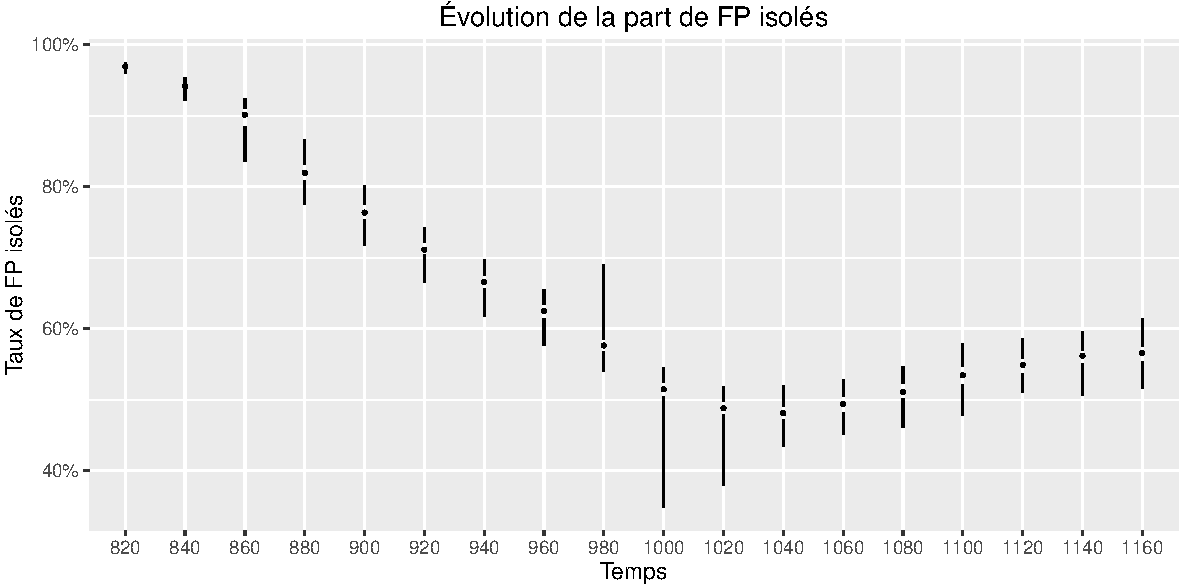
\includegraphics[width=\linewidth]{img/resultats/v0_taux_FP_isoles.pdf}
	\caption{Évolution de la part des foyers paysans isolés.} 
	\label{fig:taux-isoles-v0} 
\end{figure}

\paragraph{Nombre d'agrégats}

Puisque les foyers paysans se concentrent au sein d'agrégats, il est logique d'observer l'évolution de ces derniers. Là aussi, (\hl{objectif à définir}), on peut considérer qu'un nombre d'agrégats en fin de simulation proche de l'objectif, $200$, permet de caractériser une polarisation réussie. Cet indicateur ne peut être lu seul, et c'est pour cela qu'il vient dans un second temps (cf. p.\pageref{par:hierarchie_interne}) : en effet, un faible nombre d'agrégats peut aussi bien être révélateur d'une très faible polarisation des foyers paysans (ceux-ci restant dispersés) que d'une trop importante (un unique agrégat concentrant l'ensemble des foyers paysans par exemple).
Une fois le taux de foyers paysans dispersés connu et ces potentiels biais pris en compte, le nombre d'agrégats et son évolution nous renseigne cependant sur les dynamiques de polarisation. 
D'après les connaissances expertes, on s'attend à ce que le nombre d'agrégats, très faible au départ (24 dans la version 0), suive trois phases : une première phase de croissante lente, le temps que les mécanismes agissent sur la polarisation, suivie d'une période de croissance plus rapide, une fois que tous les foyers paysans commenceront à être suffisament attirés par les pôles pour y former des agrégats, et enfin, une nouvelle phase de croissante plus lente, une fois les foyers paysans répartis dans les agrégats existants et qui se déplaceront vers des agrégats plus importants, hiérarchisant le système de peuplement. Cette allure d'évolution rappelle les fonctions logistiques connues par exemple pour les cycles de diffusion/adoption des innovations \hl{ref Pumain ou MN Comin}, et résulte des connaissances expertes des archéologues spécialistes de la période.

\begin{mdframed}[backgroundcolor=gray!10,footnoteinside=false]
	Le nombre d'agrégats est assez satisfaisant dans la version 0 du modèle. Il s'élève ainsi à $\textbf{187}$ en moyenne, cette dernière étant d'ailleurs stable au regard des réplications. L'écart à l'objectif ($200$) est donc assez minime. On a toutefois vu que le taux de foyers paysans isolé était bien trop important, et dès lors, ces agrégats sont logiquement composés de trop peu de foyers paysans.
	
	L'observation de cet indicateur au cours du temps (\cref{fig:nombre-agregats-v0}) est quant à elle assez satisfaisante : on retrouve bien les trois phases attendues, quand bien même le début de la croissance plus importante (vers 1000 ici) est un peu trop tardive. Ce moment coïncide de plus avec la stagnation puis l'inversion de la courbe d'évolution de la part de foyers paysans isolés.
	
	On peut quand même considérer que si la polarisation n'est pas assez importante, les structures qui en résultent semblent correspondre à l'empirie.
\end{mdframed}

\begin{figure}[H]
	\captionsetup{width=\linewidth}
	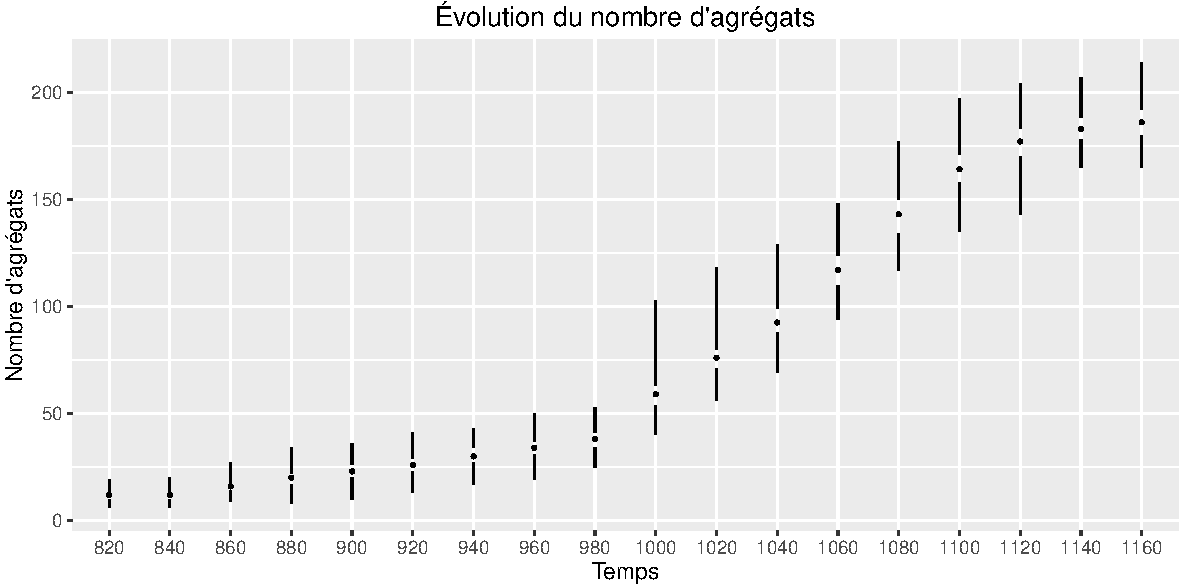
\includegraphics[width=\linewidth]{img/resultats/v0_nombre_agregats.pdf}
	\caption{Évolution du nombre d'agrégats.} 
	\label{fig:nombre-agregats-v0} 
\end{figure}

\todobox{
		Il y a un problème ici par rapport à ce qui a été mis dans le chapitre : dans le chapitre TMD, on mentionne 83 agrégats en moyenne, alors que dans l'analyse de Base, il y en a 187...
}	

\paragraph{Nombre de pôles}

Dans le modèle SimFeodal, les foyers paysans sont polarisés par des pôles d'attraction. Pour une polarisation efficace, il est donc nécessaire que les pôles soient suffisamment nombreux, c'est-à-dire, \textit{a minima}, autant que d'agrégats attendus ($200$). Contrairement aux agrégats, un nombre trop important de pôles ne constitue pas un problème : en considérant que $20\%$ des foyers paysans doivent demeurer isolés en fin de simulation, il est vraisemblable qu'une partie des pôles, par exemple composés d'une église paroissiale, n'aient pas vocation à voir la constitution d'un agrégat autour d'eux.

Par ailleurs, afin de renforcer la polarisation par l'action de l'attraction différenciée -- selon le nombre de foyers paysans contenus dans chaque agrégat\footnote{L'attraction qu'exercent les pôles contenant des agrégats de population est ainsi plus forte lorsque ces derniers sont constitués d'un nombre de foyers paysans important, et moindre quand ce nombre est faible. Cela place ce mécanisme dans une logique proche de celle de l'attachement préférentiel identifié par \autocite{yule1925ii} et  \autocite{simon1955class}, cités par \autocite[93]{schmitt_modelisation_2014-1}) \label{ftn:attachement-preferentiel}} --, il faut que le taux de pôles contenant un agrégat soit important, et surtout croissant au cours du temps : comme dans l'empirie, cela est alors le marqueur que de petits pôles d'attractions, comme les églises paroissiales, parviennent à polariser suffisament de foyers paysans de leur voisinage pour aboutir à la création d'un petit agrégat, un village par exemple.

Pour un résultat satisfaisant, il faut donc que le nombre de pôles augmente régulièrement au cours de la durée de la simulation, et que le taux de pôles contenant un agrégat augmente lui aussi de manière continue.

\begin{mdframed}[backgroundcolor=gray!10,footnoteinside=false]
	L'évolution du nombre de pôles est assez représentative de l'empirie dans la version 0 de SimFeodal. On aboutit ainsi sur $\textbf{190}$ pôles en moyenne en fin de simulation, ce qui est dans le bon ordre de grandeur, quoi qu'un peu trop faible. Ce nombre est en croissance constante à partir de 940 (\cref{fig:nombre-poles-v0}). Ce départ quelque peu tardif peut expliquer le relatif manque de pôles en fin de simulation.
	
	L'analyse de la constitution de ces pôles en matière d'agrégat est toutefois plus décevante : la croissance n'est pas linéaire, stagnant entre 940 et 1000, puis à partir de 1040. On constate ici un mauvais comportement du modèle par rapport à l'empirie : il y a création de nombreux pôles, mais ceux-ci ne suffisent pas à polariser les foyers paysans. On peut donc penser qu'il s'agit de nombreux pôles ruraux, par exemple composés d'une unique église paroissiale, ne suffisant dès lors pas à concentrer les foyers paysans alentours.
	
	Dans cette dimension, comme pour l'indicateur principal qu'en est le taux de foyers paysans dispersé, l'effet de la polarisation apparaît nettement trop faible.
\end{mdframed}


\begin{figure}[H]
	\captionsetup{width=\linewidth}
	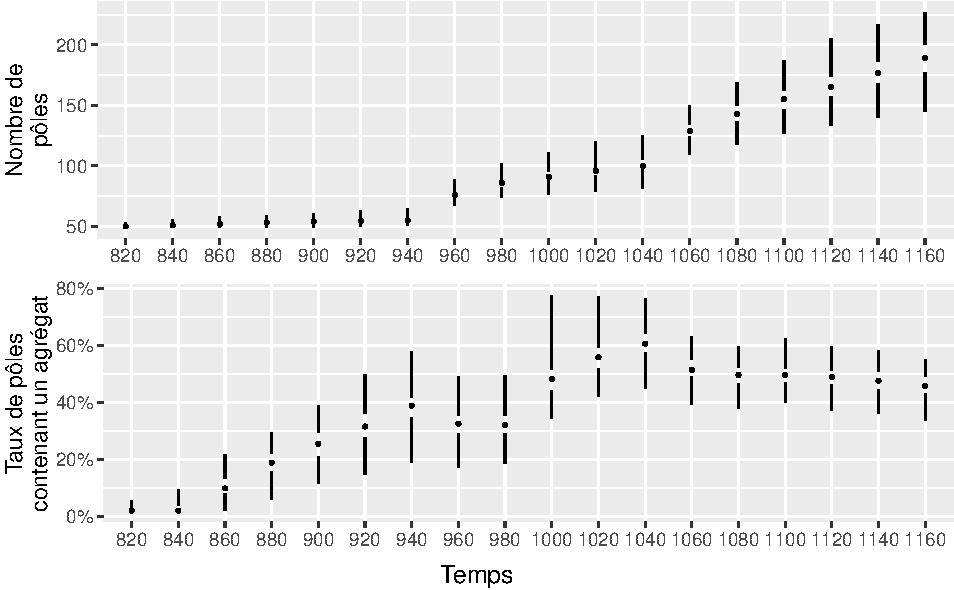
\includegraphics[width=\linewidth]{img/resultats/v0_nombre_poles.pdf}
	\caption{Évolution du nombre de pôles et du taux de pôles contenant un agrégat.} 
	\label{fig:nombre-poles-v0} 
\end{figure}

\paragraph{Dispersion des agrégats et pôles}

Les indicateurs présentés ci-dessus avaient en commun d'être des indicateurs de sortie, générés automatiquement, et présentés sous forme d'agrégations des réplications. Pour préciser l'analyse de la polarisation, il est toutefois nécessaire d'aborder une dimension qui n'est fondamentalement pas agrégeable dans les indicateurs de sortie : l'espace du modèle. Comme celui-ci est théorique et aléatoire, il n'y a aucun sens à agréger des entités différentes, par exemple des agrégats, sachant que ceux-ci occupent des localisation aléatoires et ne sont pas identifiables en tant que tels.

On ne peut cependant pas se passer d'une analyse spatiale de la répartition des pôles et agrégats afin de comprendre les dynamiques effectivement simulées par le modèle. La distribution spatiale des agrégats et des pôles est en effet un facteur majeur de la polarisation : s'ils sont très concentrés, les foyers paysans non présents alentours ne trouveront pas d'attracteurs à proximité, et ne seront de plus pas particulièrement affectés par l'augmentation des droits (banaux etc.) et des contraintes spatiales (proximité à une église, à un château etc.). A l'inverse, des agrégats entièrement dispersés ne favoriseraient pas la structure spatiale hiérarchisée que l'on chercher à faire émerger.

Afin que le comportement du modèle soit satisfaisant, il faut donc que les pôles et agrégats occupent l'ensemble de l'espace du modèle, tout en présentant des zones de concentration relatives plus importantes. Comme on ne peut agréger les représentations spatiales, il convient, pour cette analyse, de regarder individuellement un échantillon de configurations spatiales générées.

\begin{mdframed}[backgroundcolor=gray!10,footnoteinside=false]
	La lecture des cartes de répartition des agrégats et des pôles de deux réplications de la version 0 (\cref{fig:cartes-agregats-v0}) va, dans l'ensemble, dans le sens de l'empirie. On peut ainsi remarquer que ces entités ont bien tendance, au cours du temps, à se disperser dans l'espace modélisé. En fin de simulation, tout l'espace est occupé, et on remarque même que certaines zones voient une forte concentration en agrégats, reproduisant les faits stylisés connus. La répartition spatiale des agrégats -- et des pôles -- est donc bonne, et ne semble pas opposer d'obstacle à la polarisation attendue du système de peuplement.
	
	Ce résultat peut cependant être nuancé par l'observation de la dynamique de cette dispersion : on constate ainsi que la dispersion s'effectue rapidement (entre 800 et 940), et n'évolue plus vraiment après. Ce phénomène est donc plus rapide dans cette version 0 du modèle que dans les connaissances empiriques de la région Touraine.
	
	On peut enfin remarquer, en préalable aux dynamiques de hiérarchisation du système que l'on s'apprête à étudier, que ces sorties illustrent un manque criant de hiérarchie quant à la composition des agrégats : on ne remarque, visuellement, que peu de différence entre les agrégats, et surtout, cette hiérarchie semble faiblir entre 1040 et 1160 (les agrégats les plus importants ont vu leur nombre de foyers paysans diminuer).
\end{mdframed}

\begin{figure}[H]
	\captionsetup{width=\linewidth}
	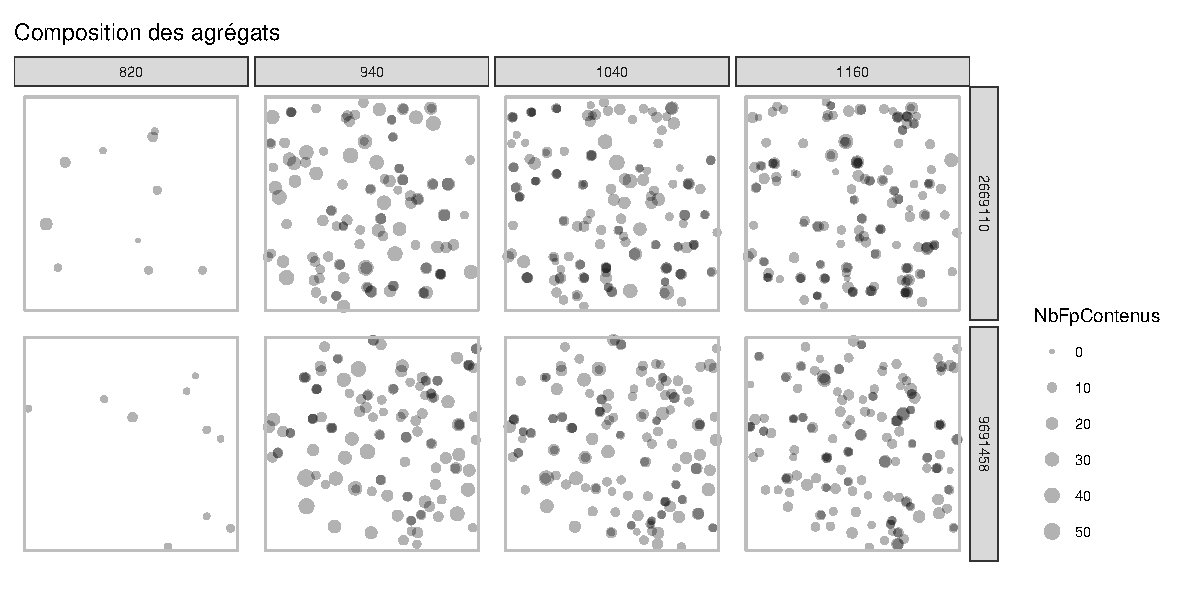
\includegraphics[width=.47\linewidth]{img/resultats/v0_cartes_agregats.pdf}
	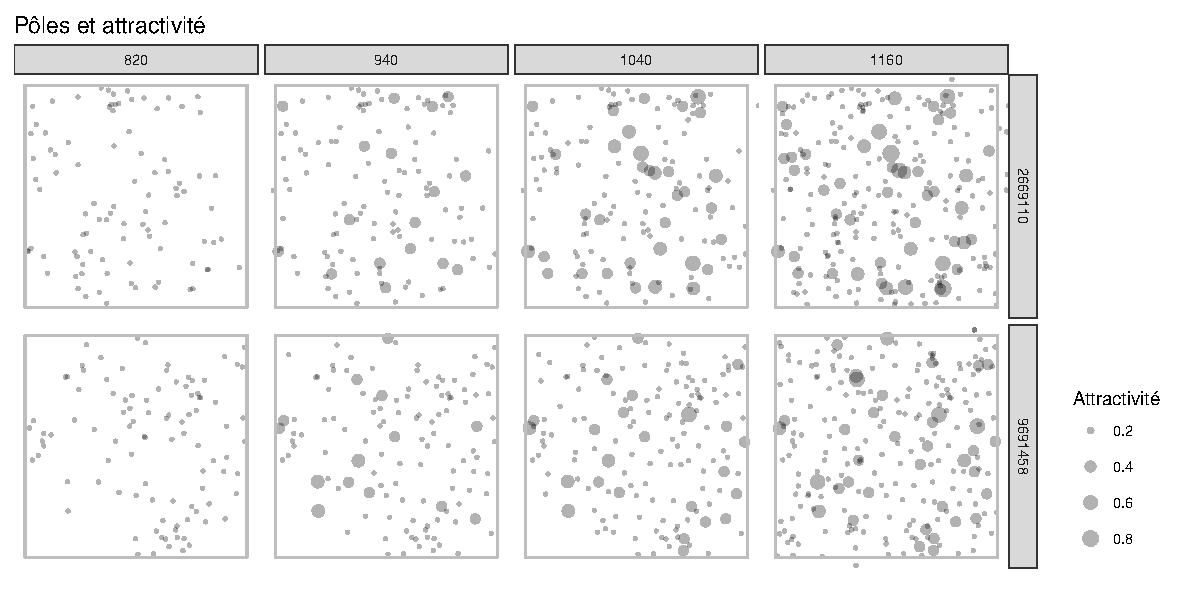
\includegraphics[width=.47\linewidth]{img/resultats/v0_cartes_poles.pdf}
	\caption{Évolution de la répartition spatiale des agrégats et pôles, pour deux réplications.} 
	\label{fig:cartes-agregats-v0} 
\end{figure}

\subsubsection{Évaluer la hiérarchisation du système de peuplement}

Le second grand fait stylisé que l'on cherche à reproduire dans SimFeodal correspond à une forte hiérarchisation du système de peuplement et plus généralement, des entités présentes. On passe ainsi, en 800, d'un habitat dispersé dans lequel coexistent quelques agrégats de taille uniforme, à un habitat concentré dans des agrégats de taille très hétérogènes. La distribution des tailles des agrégats est estimée par les connaissances expertes, toutes proportions gardées, comme assez proche des distributions observées aujourd'hui dans les systèmes de peuplement.
On souhaite ainsi que les agrégats modélisés suivent une distribution approchant la distribution log-normale.

Par extension, et là encore d'après les connaissances thématiques, l'ensemble des entités doit aussi suivre le même type de forme. Par exemple, les pôles, tant en terme d'attractivité que de composition, doivent aussi montrer une hiérarchie du même ordre, ainsi que les seigneurs -- à travers leur puissance, au moins pour les petits seigneurs --, ou encore les paroisses, par le nombre de paroissiens qu'elles desservent.

Comme pour l'étude de la polarisation, on peut définir un indicateur principal de cette hiérarchisation du système de peuplement : la forme de la distribution de la composition en foyers paysans des agrégats.

De la même manière que pour la polarisation, les indicateurs secondaires ont aussi pour but de préciser cet indicateur principal, et en particulier d'analyser les moteurs de cette hiérarchisation du peuplement.
On a en effet choisi d'observer plutôt la hiérarchisation des autres types d'entités -- pôles, seigneurs, paroisses --, pour vérifier qu'elles accompagnent et/ou entraînent bien la hiérarchisation des agrégats. La hiérarchie des pôles, par exemple, a une influence directe sur l'attraction effectuée sur les foyers paysans (polarisation) et sur la hiérarchisation des agrégats : par effet d'attraction différenciée (voir la note de bas de page \ref{ftn:attachement-preferentiel} \cpageref{ftn:attachement-preferentiel}), des agrégats plus importants se constituent autour des pôles les plus importants.

Comme pour la polarisation, l'analyse de la capacité du modèle a reproduire la hiérarchisation du système de peuplement se fait donc en deux temps : en premier lieu, on évalue cette capacité à l'aide de l'indicateur principal, puis on précise cette qualification et on essaie de l'expliquer à l'aide des indicateurs secondaires.


\paragraph{Hiérarchie des agrégats}

L'indicateur principal est un indicateur agrégé, correspondant à la forme de la distribution des agrégats mesurés par le nombre de foyers paysans qui les composent. Cet indicateur est classique dans l'analyse des systèmes de peuplement, et il est courant de l'observer par le biais d'un indicateur agrégé simple, correspondant à la loi rang-taille. On observe pour cela le modèle statistique, ou sa représentation graphique tout du moins, mettant en relation le logarithme de la taille des individus (le nombre de foyers paysans composant chaque agrégat ici) et le logarithme du rang de cet individu. Comme pour toute régression linéaire, on peut alors quantifier l'ajustement du modèle grâce au coefficient de détermination ($R^2$), et spécifier la pente de la courbe, représentant le degré de hiérarchie, à travers le coefficient directeur ($a$ dans la formule $y = ax + b$).

Dans le cas de SimFeodal, le faible nombre d'agrégats ainsi que la variabilité de leurs tailles rend difficile cette analyse quantifiée, le coefficient directeur, par exemple, étant très sensible aux faibles effectifs. On utilise toutefois la représentation graphique décrite comme un indicateur majeur de la hiérarchie des agrégats.

Du point de vue des connaissances empiriques, la courbe doit ainsi voir sa pente augmenter avec le temps, tout en devenant plus convexe, ce qui représente la \og longue traine\fg{} des petits agrégats, empiriquement observée dans toutes les distributions de systèmes de peuplement.

Avec une autre représentation graphique du même phénomène, en discrétisant les agrégats selon leur taille et en dénombrant le nombre d'agrégats de chaque classe, on peut aussi avoir une vision plus synthétique (car moins exhaustive) de la forme de la distribution. On doit alors obtenir un nombre décroissant d'agrégats à mesure que la classe représente un nombre élevé de foyers paysans.

\todobox{
		Ça vaudrait peut-être le coup, pour chaque indicateur présenté sous forme graphique (évolution ou forme), de faire un graphique théorique (une sorte de courbe parfaite) de ce que l'on souhaite observer.
		}

\begin{mdframed}[backgroundcolor=gray!10,footnoteinside=false]
	La version 0 de SimFeodal présente une hiérarchisation des agrégats nettement trop faible. La courbe rang-taille (\cref{fig:rt-agregats-v0}) est ainsi trop faiblement pentue, et présente une forme trop linéaire : la convexité due à la longue traine n'est pas assez visible, en raison sans doute de trop faibles valeurs  en haut de la hiérarchie, qui ne \og tire\fg{} alors pas assez la distribution.
	Ce résultat de simulation est d'autant plus perturbant que son évolution est éloignée de l'empirie : on remarque en effet que la distribution se hiérarchise bien entre 800 et 1020, présentant à cette date une allure très satisfaisante. Pourtant, après cette période, les agrégats voient leur hiérarchie diminuer nettement et les agrégats les plus peuplés diminuer en taille.
	
	On constate le même décrochage dans la discrétisation des agrégats (\cref{fig:compo-agregats-v0}), où on remarque de plus que la hiérarchie la plus proche de l'attendu, où la position des classes suivrait une ligne droite, semble se dessiner entre 940 et 1040. En 1040, et plus encore en 1160, la proportion d'agrégats de taille moyenne et haute (de 30 à 100, et de plus de 100 foyers paysans) est trop faible, et pas assez hiérarchisée.
	
\end{mdframed}

\begin{figure}[H]
	\captionsetup{width=\linewidth}
	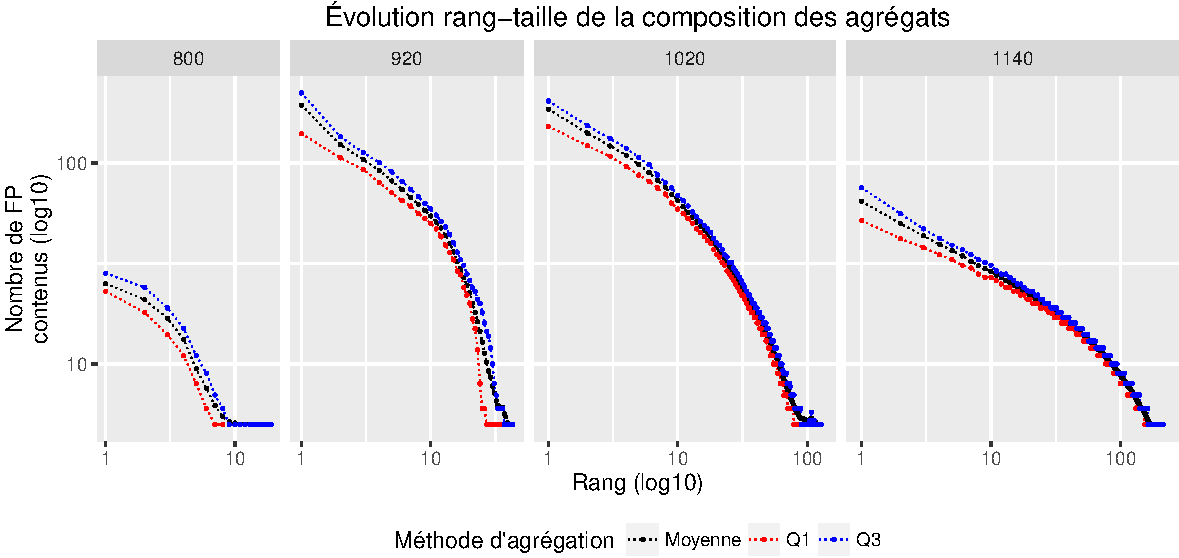
\includegraphics[width=.8\linewidth]{img/resultats/v0_rt_agregats.pdf}
	\caption{Évolution de la courbe rang-taille des agrégats.} 
	\label{fig:rt-agregats-v0} 
\end{figure}

\begin{figure}[H]
	\captionsetup{width=\linewidth}
	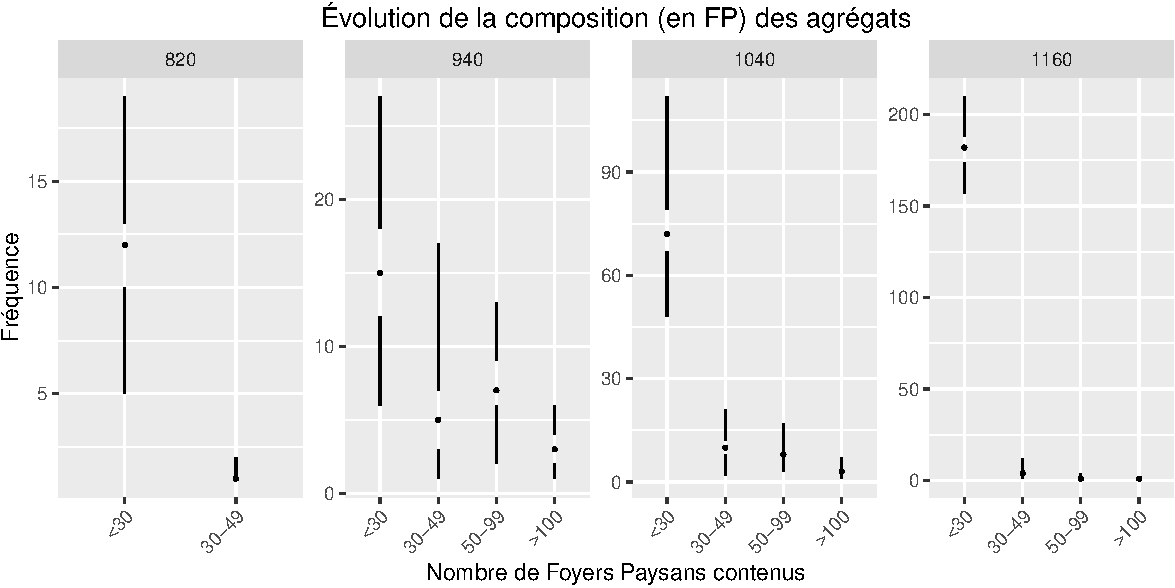
\includegraphics[width=.8\linewidth]{img/resultats/v0_compo_agregats.pdf}
	\caption{Évolution de la composition des agrégats.} 
	\label{fig:compo-agregats-v0} 
\end{figure}

\paragraph{Hiérarchie des pôles}

\begin{mdframed}[backgroundcolor=gray!10,footnoteinside=false]
	(\cref{fig:compo-poles-v0})
\end{mdframed}

\begin{figure}[H]
	\captionsetup{width=\linewidth}
	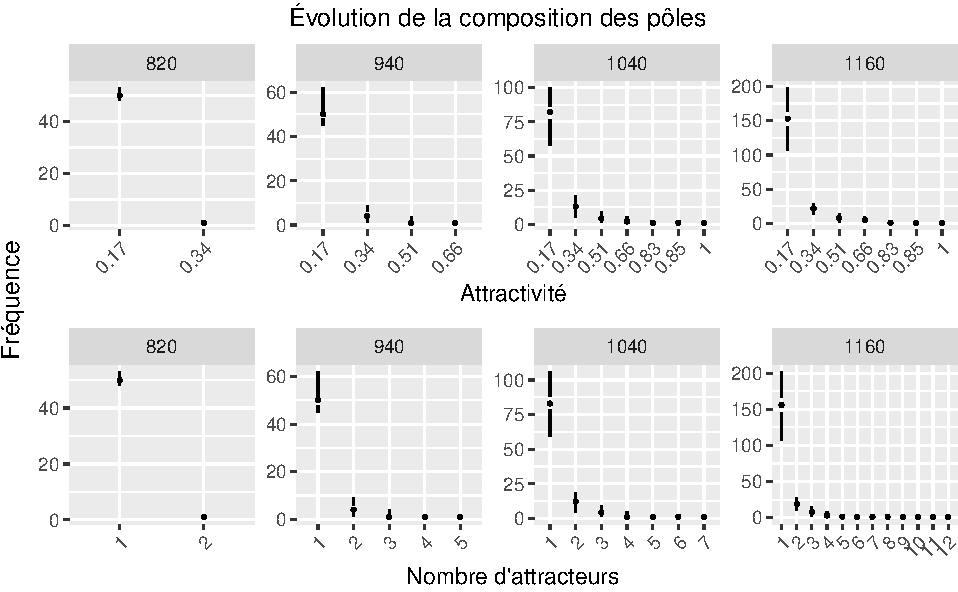
\includegraphics[width=\linewidth]{img/resultats/v0_compo_poles.pdf}
	\caption{Évolution de la composition et de l'attractivité des pôles.} 
	\label{fig:compo-poles-v0} 
\end{figure}

\paragraph{Hiérarchie des paroisses}

\begin{mdframed}[backgroundcolor=gray!10,footnoteinside=false]
	(\cref{fig:compo-paroisses-v0})
\end{mdframed}

\begin{figure}[H]
	\captionsetup{width=\linewidth}
	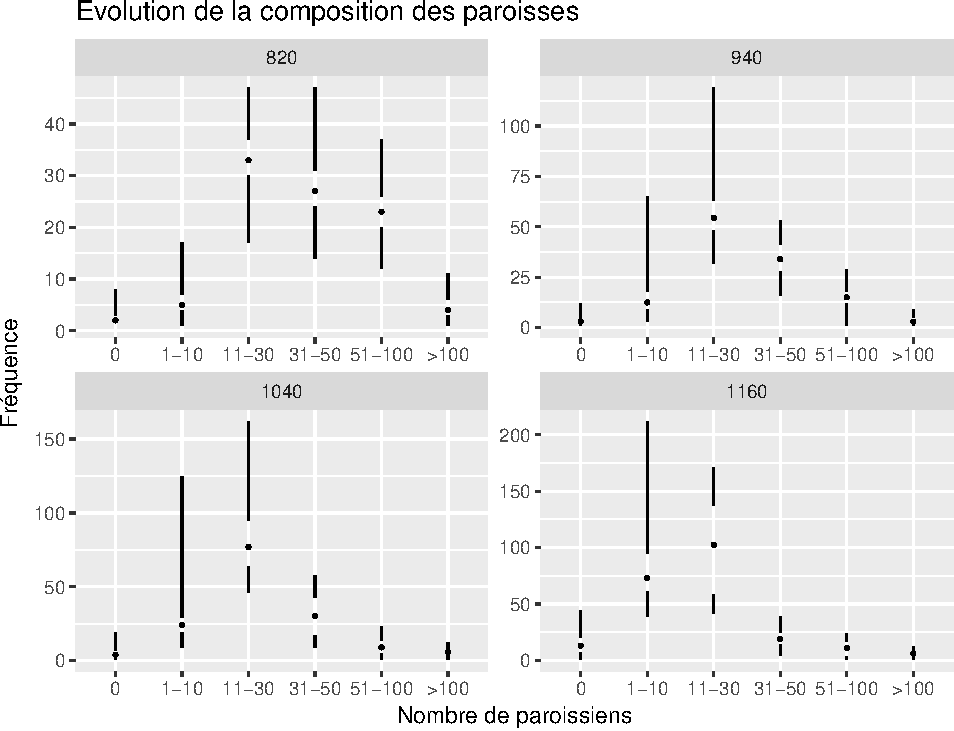
\includegraphics[width=\linewidth]{img/resultats/v0_compo_paroisses.pdf}
	\caption{Évolution de la composition des paroisses.} 
	\label{fig:compo-paroisses-v0} 
\end{figure}



\subsubsection{Évaluer la fixation et la dissémination du peuplement}

%\paragraph{Stabilité}


\todobox{		
		\begin{itemize}
			\item \textbf{Polarisation} : il faut qu'ils rassemblent les FP (taux isolés faible),
			\item \textbf{Hiérarchisation} : qu'ils soient hiérarchisés (composition des agrégats en FP doit tendre vers log-normale),
			\item \textbf{Fixation et dispersion} : et qu'ils soient dispersés dans l'espace de manière stable (fixation par paroisses).
		\end{itemize}
		
		3 leviers différents pour jouer sur ces dimensions :
		\begin{itemize}
			\item \textbf{Polarisation} : Améliorer le déplacement des FP (Agent concerné : FP) :
			\begin{itemize}
				\item ils doivent se déplacer vers un petit agrégat/pôle et ne pas rester isolés
				\item une fois dans un agrégat, ils doivent y rester ou aller vers un agrégat plus \og important\fg{} : en terme de nb de FP, d'attractivité du pôle ou de présence de CA
				\item Ils ne doivent pas faire des allers-retours incessants entre les agrégats.
			\end{itemize}
			
			\item \textbf{Hiérarchisation} : Améliorer la hiérarchisation des attracteurs (Agent concerné : Attracteurs) :
			\begin{itemize}
				\item La différence entre les pôles d'attraction doit être franche,
				\item pour que les petits (1 église par ex.) attirent de petits agrégats,
				\item et que les gros (châteaux, multi-pôles etc.) polarisent des agrégats importants et stables
			\end{itemize}
			\item \textbf{Fixation et dispersion} : Améliorer la desserte des églises paroissiales (Agent concerné : Paroisse) :
			\begin{itemize}
				\item Les paroisses doivent couvrir tout le territoire de manière à peu près régulière (logique d'équité),
				\item Mais aussi avec des zones de plus forte densité proche des gros pôles/agrégats (petites villes) (logique d'efficacité),
			\end{itemize}
			
		\end{itemize}
}	
